\documentclass[conference]{IEEEtran}
\IEEEoverridecommandlockouts

% Packages
\usepackage{cite}
\usepackage{amsmath,amssymb,amsfonts}
\usepackage{graphicx}
\usepackage{textcomp}
\usepackage{listings}
\usepackage{subcaption}
\usepackage{float}
\usepackage{multirow}
\usepackage{algorithm}
\usepackage{algpseudocode}
\usepackage{algorithmicx}
\usepackage{url}
\usepackage{caption}
\usepackage{tcolorbox}
\usepackage{hyperref}
\usepackage[T1]{fontenc}
\usepackage{enumitem}
\usepackage{multicol}
\usepackage{enumitem}
\usepackage{balance}
\usepackage{array,booktabs}
\usepackage{stackengine}

\newcommand{\myvec}[1]{\ensuremath{\begin{matrix}#1\end{matrix}}}
\DeclareMathAlphabet\mathbfcal{OMS}{cmsy}{b}{n}

\setlength {\marginparwidth }{2cm}
\newlength{\subfigwidth}
\setlength{\subfigwidth}{0.2\textwidth}
\newcolumntype{M}[1]{>{\centering\arraybackslash}m{#1}} % w/ horizontal centering

% Macro for growth comparison row
\newcommand{\growthcomparisonrow}[6]{%
    #1 &
    \begin{subfigure}[b]{\subfigwidth}
        \includegraphics[width=\textwidth]{figures/growth_comparison_lambda_#2/#1.#3.png}
    \end{subfigure} &
    \begin{subfigure}[b]{\subfigwidth}
        \includegraphics[width=\textwidth]{figures/growth_comparison_lambda_#2/#1.#4.png}
    \end{subfigure} &
    \begin{subfigure}[b]{\subfigwidth}
        \includegraphics[width=\textwidth]{figures/growth_comparison_lambda_#2/#1.#5.png}
    \end{subfigure} &
    \begin{subfigure}[b]{\subfigwidth}
        \includegraphics[width=\textwidth]{figures/growth_comparison_lambda_#2/#1.#6.png}
    \end{subfigure}  \\
}


\hypersetup{hidelinks}

\tcbuselibrary{listingsutf8}
\newtcbox{\redbox}[1][]{
 on line, 
 boxsep=1pt, 
 left=1pt, 
 right=1pt, 
 top=1pt, 
 bottom=1pt, 
 colframe=red!75!black, 
 colback=red!10, 
 boxrule=0.5pt, 
 rounded corners,
 #1
}

\algrenewcommand\algorithmicindent{0.8em} 



\stackMath
\newlength\matfield
\newlength\tmplength
\def\matscale{1.}
\newcommand\dimbox[3]{%
  \setlength\matfield{\matscale\baselineskip}%
  \setbox0=\hbox{\vphantom{X}\smash{#3}}%
  \setlength{\tmplength}{#1\matfield-\ht0-\dp0}%
  \fboxrule=1pt\fboxsep=-\fboxrule\relax%
  \fbox{\makebox[#2\matfield]{\addstackgap[.5\tmplength]{\box0}}}%
}
\newcommand\raiserows[2]{%
   \setlength\matfield{\matscale\baselineskip}%
   \raisebox{#1\matfield}{#2}%
}
\newcommand\matbox[5]{
  \stackunder{\dimbox{#1}{#2}{$#5$}}{\scriptstyle(#3\times #4)}%
}

\begin{document}

\title{Proliferating Cell Collectives: \\A Comparison of Hard and Soft Collision Models}

\author{
    \IEEEauthorblockN{Manuel Lerchner}
    \IEEEauthorblockA{
        \textit{Technical University of Munich}\\
        Munich, Germany}
}

\maketitle

\begin{abstract}
    This thesis investigates the computational modeling of proliferating cell collectives, focusing on the fundamental differences between hard (constraint-based) and soft (potential-based) collision models. Building on recent advances in understanding bacterial colony pattern formation \cite{Weady2024}, we demonstrate that both approaches can reproduce the experimentally observed patterns. However, we show that the soft collision model faces inherent limitations in handling growth events and maintaining proper particle spacing.

\end{abstract}

\begin{IEEEkeywords}
    active matter, cell collectives, particle simulation, constraint optimization, pattern formation, computational biology
\end{IEEEkeywords}


\section{Introduction}
\subsection{Biological Motivation}
\begin{itemize}
    \item Cell collectives and pattern formation in nature
    \item Experimental observations of bacterial colony growth
    \item Importance of understanding collective behavior
\end{itemize}

\newpage

\subsection{Computational Challenges}
\begin{itemize}
    \item Modeling proliferating active matter systems
    \item Trade-offs between computational efficiency and accuracy
    \item Time scale separation in growing systems
\end{itemize}

\newpage

\subsection{Research Questions}
\begin{itemize}
    \item Comparison of hard vs. soft collision models
    \item Impact of model choice on pattern formation
    \item Computational performance considerations
\end{itemize}

\newpage

\section{Background and Literature Review}


\subsection{Proliferating Active Matter}
\begin{itemize}
    \item Theoretical foundations of growing active matter systems
    \item Key differences from static particle systems
    \item The Weady et al. framework for pattern formation
    \item Mechanically driven growth in confined spaces
\end{itemize}

\newpage

\subsection{Collision Models}
\begin{itemize}
    \item Hard collision approaches
    \item Soft collision methods
    \item Known limitations
\end{itemize}

\newpage

\subsection{Cell Mechanics}
\begin{itemize}
    \item Rigid vs. deformable assumptions
    \item Experimental evidence
    \item Model selection implications
\end{itemize}

\newpage

\section{Mathematical Formulations}

\subsection{Common Framework}


For the reimplementation of the hard collision model, we closely follow the approach of Weady et al. \cite{Weady2024} described in the supplementary material.

Therefore we represent the current colony as a column vector $\mathbfcal{C} = [\dots, x_n^T, w_n^T, \dots]^T \in \mathbb{R}^{7N}$ where $N$ is the number of cells in the colony. Each particle is thus represented by a 7-dimensional vector consisting of a position vector $x_n \in \mathbb{R}^3$ and a unit quaternion $q_n \in \mathbb{R}^4$ representing the cell's orientation.

We determine the resulting translational and angular velocity for particles in the colony by using the force-velocity relation $\mathbfcal{U} = \mathbfcal{M} \mathbfcal{F}$, where $\mathbfcal{F}$ is the generalized force vector consisting of both force and torque components for the whole colony and $\mathbfcal{M}$ is the mobility matrix. Similar to $\mathbfcal{C}$, $\mathbfcal{U}$ and $\mathbfcal{F}$ are also stacked collumn vectors, where $\mathbfcal{F} = [\dots, f_n^T, t_n^T, \dots]^T \in \mathbb{R}^{6}$ represents the force and torque for the $n$-th cell, $\mathbfcal{M} = \text{diag}([\dots, l_n, a_n, \dots]) \in \mathbb{R}^{6 \times 6}$ is a diagonal matrix consisting of the inverse of the cell's linear and angular mobility on the diagonal and $\mathbfcal{U} = [\dots, u_n^T, \omega_n^T, \dots]^T \in \mathbb{R}^{6}$ represents the resulting translational and angular velocity for the $n$-th cell.

Combined with a map $\mathbfcal{G}$ mapping cartesian translational and angular velocities from $\mathbb{R}^{6N}$ to the corresponding change in position and quaternion in $\mathbb{R}^{7N}$, described in \cite{Weady2024}, we can express the resulting colony state after applying force and torque $\mathbfcal{F}$ for a time step $\Delta t$ as

$$
    \mathbfcal{C}^{k+1}  = \mathbfcal{C}^k + \Delta t \, \mathbfcal{G}^k\mathbfcal{U} = \mathbfcal{C}_k + \Delta t \, \mathbfcal{G}\mathbfcal{M} \mathbfcal{F}
$$
\label{eq:colony_update}

Now we can define the specific implementations of hard and soft collision models by specifying how the force vector $\mathbfcal{F}$ is computed in each case.

\newpage

\subsection{Soft Collision Model}

For the soft collision model, we use a potential-based approach inspired by \cite{Warren2019} where overlapping cells exert repelling forces on each other based on a predefined potential function. In particular, we implement a Hertzian potential, which provides a smooth force response as particles approach each other.

We use the following Model:

$$
    F_{elastic} = R_{eff} k \left( k \delta^{1.5} + \alpha \delta \right)
$$

where $R_{eff} = \sqrt{\frac{R_1 R_2}{R_1 + R_2}}$ is the effective radius of the two interacting particles with radii $R_1$ and $R_2$, $\delta$ is the overlap distance between the particles, $k$ is the elastic constant, and $\alpha$ is a linear spring coefficient used to make the particles act stiffer at small overlaps. From empirical tests, we found that setting $\alpha = 1$ and $k = 2000$ produces similar results to the hard collision model (see \autoref{fig:hertzian_contact_model}).

The overlap distance $\delta$ is calculated as the distance between the two closest points on the surface of the two particles minus the sum of their radii. If the particles are not overlapping, $\delta$ is set to zero. The resulting torque vector is then calculated as $\mathbf{T} = \mathbf{y} \times \mathbf{F}$ where $\mathbf{y}$ is the vector from the particle's center to the point of contact.

By aggregating the forces and torques from all overlapping particle pairs, we can construct the full force vector $\mathbfcal{F} = [ \dots, F_n^T, T_n^T, \dots]^T$ for the whole colony and use \autoref{eq:colony_update} to update the colony state.

\begin{figure}[H]
    \centering
    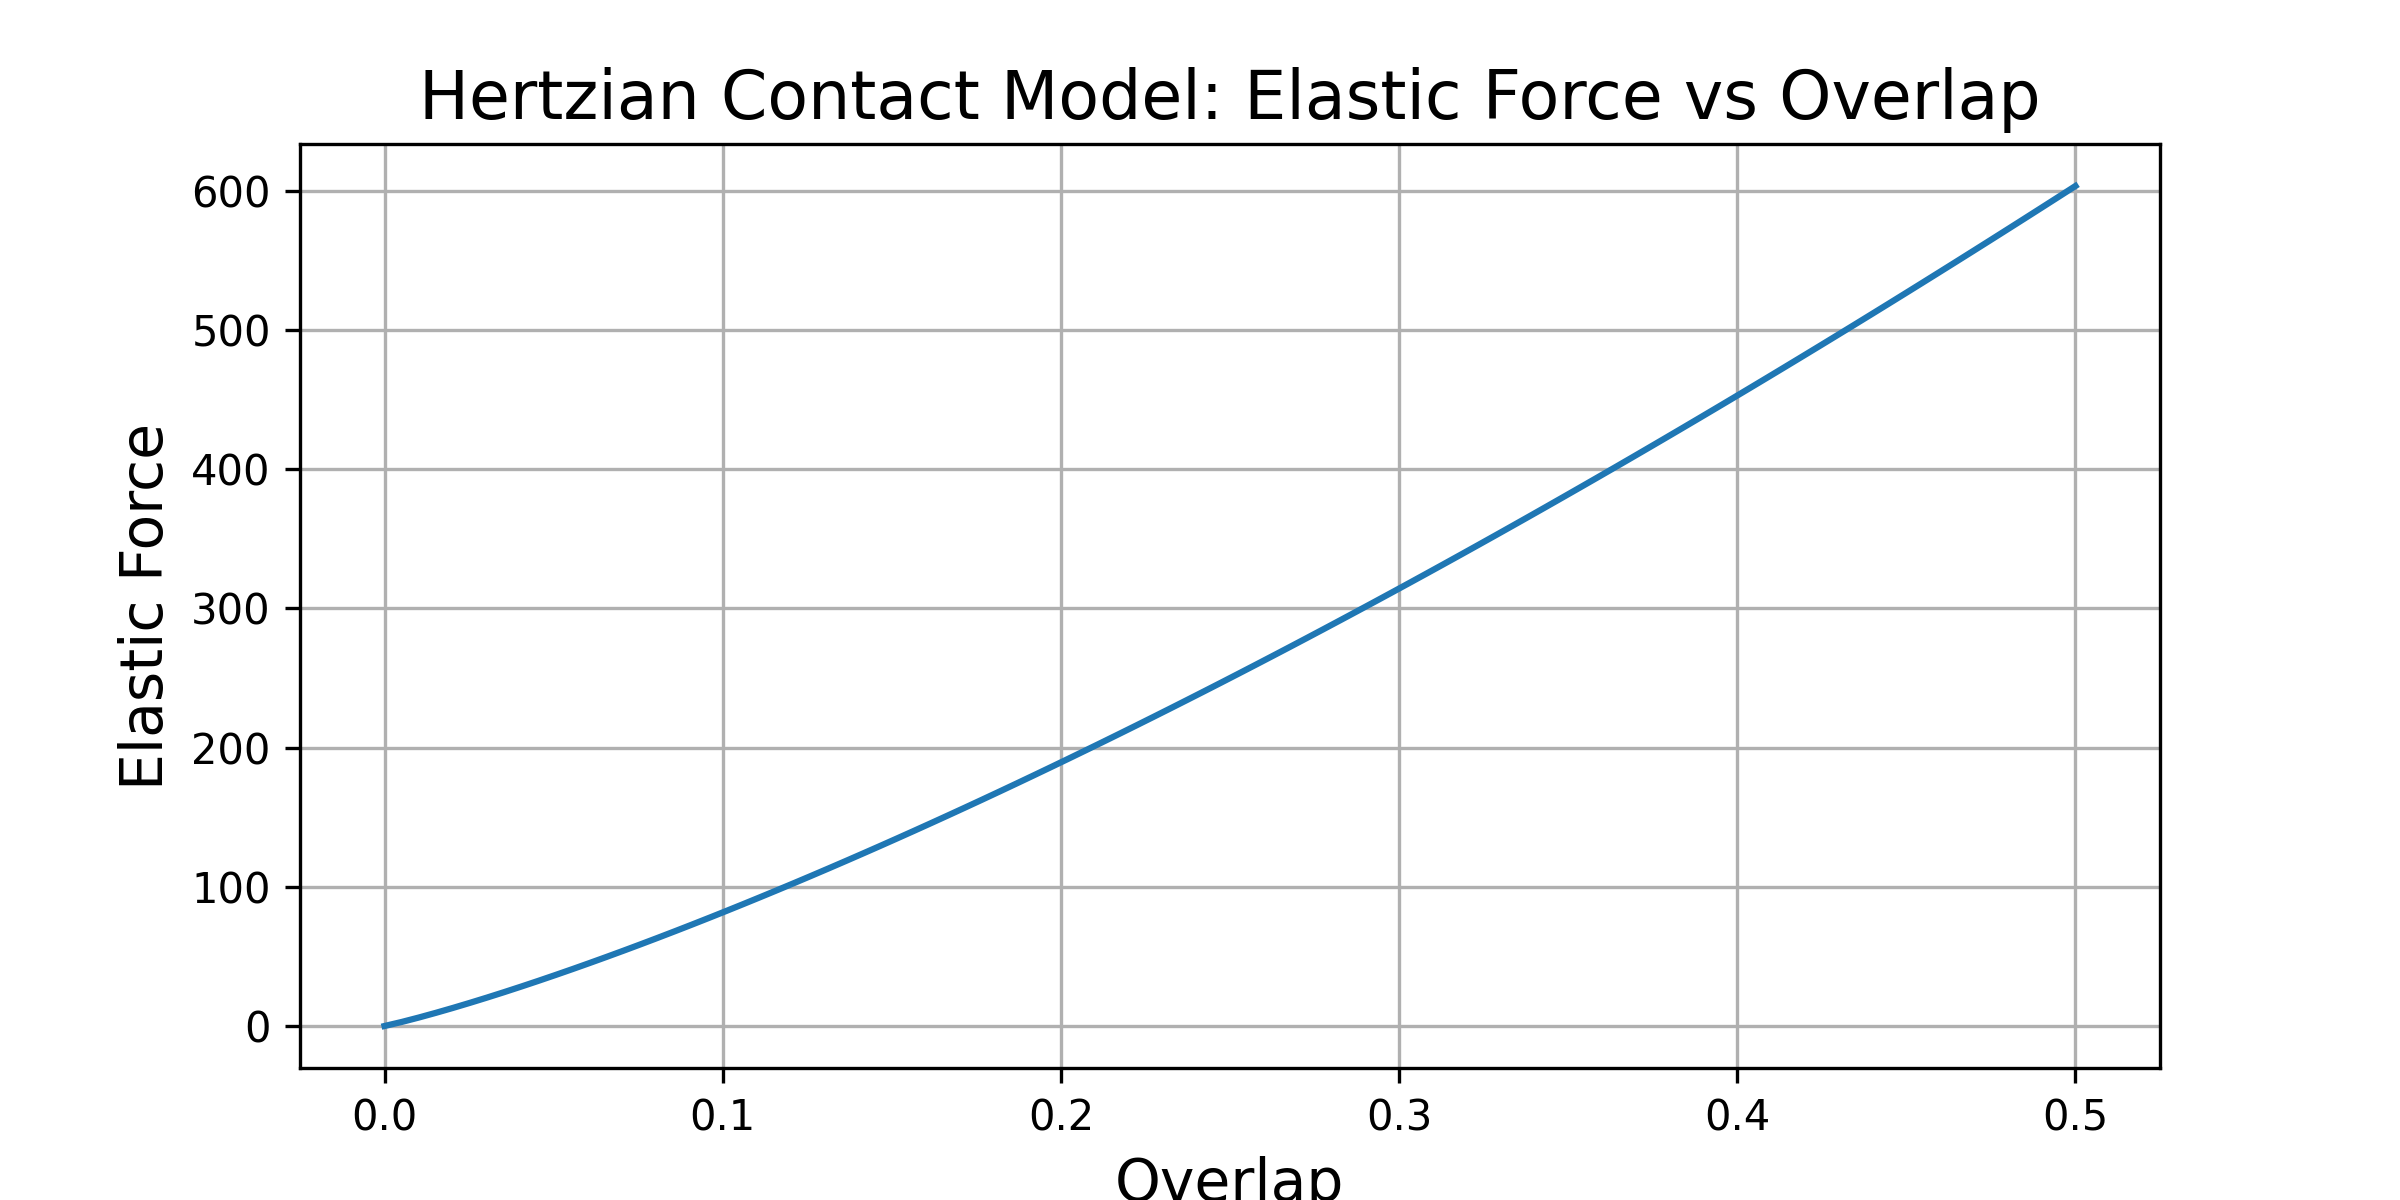
\includegraphics[width=\linewidth]{figures/hertzian_contact_model.png}
    \caption{Elastic force as a function of overlap distance for the implemented Hertzian contact model with $k=2000$ and $\alpha=0.5$.}
    \label{fig:hertzian_contact_model}
\end{figure}

\newpage
\subsection{Hard Collision Model}


For the hard collision model, we want to enforce non-overlapping constraints between cells using a constraint-based approach. Therefore we create a constraint $\alpha$ for each pair of nearby cells consisting of the two closest points $\mathbf{y}_n$ and $\mathbf{y}_m$ on the surfaces of the two particles.

The applied force and torque of such a constraint $\alpha$ on a particle $n$ can then be expressed as:

$$
    \mathbf{F}_\alpha^n = - \hat{\mathbf{n}}_\alpha ^n \gamma_\alpha \in \mathbb{R}^3, \qquad \mathbf{T}_\alpha^n = \mathbf{y}_n \times \mathbf{F}_\alpha^n \in \mathbb{R}^3
$$
\label{eq:constraint_force}

where $\hat{\mathbf{n}}_\alpha ^n$ is the normal vector at point $\mathbf{y}_n$ pointing away from the other particle and $\gamma_\alpha$ is the yet unknown Lagrange multiplier associated with constraint $\alpha$ representing the magnitude of the force needed to satisfy the non-overlapping condition.

By aggregating the contributions from all constraints $A_n$ affecting the $n$-th particle, we can express the combined force and torque on a particle as:

$$
    \mathbf{F}_n = \sum_{\alpha \in A_n} \mathbf{F}_\alpha^n, \qquad \mathbf{T}_n = \sum_{\alpha \in A_n} \mathbf{T}_\alpha^n
$$
\label{eq:total_force}

From those two components for each particle, we can construct the full force vector $\mathbfcal{F} = [ \dots, F_n^T, T_n^T, \dots]^T$ for the whole colony and use \autoref{eq:colony_update} to update the colony state.


\subsection{Lagrange Multiplier Calculation}

The equations presented in \autoref{eq:colony_update} and \autoref{eq:constraint_force} depend on the unknown Lagrange multipliers $\gamma_\alpha$ for each constraint $\alpha$. This factor scales each constraint force to ensure that the non-overlapping conditions are satisfied after each update step, i.e., that no two particles overlap.

To simplify the notation we combine all lagrange multplieres $\gamma_\alpha$ into a single vector $\mathbf{\gamma} = [\dots, \gamma_\alpha, \dots]^T \in \mathbb{R}^{C}$ where $C$ is the total number of constraints in the system. Moreover we define a signed seperation distance function $\Phi_{\alpha}$ for each constraint $\alpha$ such that $\Phi_{\alpha} > 0$ if the two particles are separated, $\Phi_{\alpha} = 0$ if they are just touching and $\Phi_{\alpha} < 0$ if they are overlapping. Again we simplify the notation by combining all seperation distances into a single vector $\mathbf{\Phi} = [\dots, \Phi_\alpha, \dots]^T \in \mathbb{R}^{C}$.


\subsection{Constraints}

We only ever want repelling forces, i.e., $\gamma_\alpha \geq 0$ for all constraints $\alpha$, and require $\Phi_{k}^{k+1} \geq 0$ after the update step to ensure that all particle overlaps are resolved. Moreover we only want to apply forces for constraints where $\Phi_{\alpha} < 0$ to resolve overlaps and need $\gamma_\alpha = 0$ otherwise to ensure that non-overlapping particles do not exert forces on each other. This is elegantly expressed by the complementarity condition $\mathbf{\Phi} \bot \mathbf{\gamma} = \mathbf{\Phi}^T \mathbf{\gamma}$ which states that for each constraint $\alpha$ if the particles are not overlapping ($\Phi_\alpha \geq 0$) then the corresponding force magnitude must be zero ($\gamma_\alpha = 0$) or if there is a non-zero force ($\gamma_\alpha > 0$) then the particles must be in contact ($\Phi_\alpha = 0$).

This can be expressed as the conditions:

$$
    \begin{align}
        \text{Positivity of multipliers:} \qquad  0 & \leq \gamma        \\
        \text{Non-overlapping condition:} \qquad  0 & \leq \Phi^{k+1}    \\
        \text{Complementarity condition:} \qquad  0 & = \gamma \bot \Phi
    \end{align}:
$$

which is often abreviated as $\mathbf{0} \leq \mathbf{\gamma} \perp \mathbf{\Phi} \geq \mathbf{0}$.


The combined update rule in \autoref{eq:colony_update} and the constraint conditions above can be combined into a single system of equations to solve for the unknown Lagrange multipliers $\mathbf{\gamma}$:

$$
    \begin{align}
        \mathbfcal{C}^{k+1} & = \mathbfcal{C}^k + \Delta t \, \mathbfcal{G}\mathbfcal{M} \mathbfcal{D}(\mathbf{\gamma}) \\
        \text{s.t.} 0       & \leq \mathbf{\gamma} \perp \mathbf{\Phi}^{k+1} \geq 0
    \end{align}
$$

Where $\mathbfcal{D} \in \mathbb{R}^{6N \times C}$ is a matrix consisting of the normal vectors $\hat{\mathbf{n}}_\alpha$ and torque arms $\mathbf{y}_n \times \hat{\mathbf{n}}_\alpha$ for each constraint $\alpha$ and particle $n$. The multiplication $\mathbfcal{D}\mathbf{\gamma}$ thus computes the total force and torque on each particle from all constraints as described in \autoref{eq:total_force}.


As $\mathbf{\Phi}^{k+1}$ is difficult to express directly as it depends on the updated colony state $\mathbfcal{C}^{k+1}$ which itself depends on $\mathbf{\gamma}$, we approximate it using a first-order Taylor expansion around the current state $\mathbfcal{C}^k$:

$$
    \mathbf{\Phi}^{k+1} \approx \mathbf{\Phi}^k + \Delta t \mathbf{D}^k \dot{\mathbfcal{C}^k} = \mathbf{\Phi}^k + \Delta t \mathbf{D}^k \mathbfcal{G}^k \mathbfcal{M} \mathbfcal{D} \mathbf{\gamma}
$$

The resulting system of equations to solve for $\mathbf{\gamma}$ is thus:

$$
    \begin{align}
        \mathbfcal{C}^{k+1} & = \mathbfcal{C}^k + \Delta t \, \mathbfcal{G}\mathbfcal{M} \mathbfcal{D}(\mathbf{\gamma})                                                            \\
        \text{s.t.} 0       & \leq \mathbf{\gamma} \perp \left( \mathbf{\Phi}^k + \Delta t \mathbf{D}^k \mathbfcal{G}^k \mathbfcal{M} \mathbfcal{D} \mathbf{\gamma} \right) \geq 0
    \end{align}
$$


This set of conditions is known as a Linear Complementarity Problem (LCP) and the missing Lagrange multipliers $\mathbf{\gamma}$ can be solved for using various numerical methods such as the the BBPGD algorithm described in \cite{Weady2024}. This allows us to compute the exact forces needed to resolve all overlaps in a single update step (excluding approximation errors from the Taylor expansion), ensuring that the non-overlapping conditions are satisfied at all times.




\newpage

\section{Implementation and Results}
\subsection{Simulation Framework}
\begin{itemize}
    \item Implementation details
    \item Data structures
    \item Performance optimization
\end{itemize}

\newpage

\subsection{Pattern Formation Analysis}

To analyze the pattern formation capabilities of both hard and soft collision models under stress-sensitive growth, aswell as to verify our implementation, we reproduce the concentric ring patterns observed by Weady et al. \cite{Weady2024}. We conduct simulations for three different values of the stress sensitivity parameter $\lambda$ ($10^{-1}$, $10^{-2}$, and $10^{-3}$) for both collision models. The results are presented in \autoref{fig:pattern_formation}.

The patterns formed by both models closely resemble those reported by Weady et al., confirming the validity of our implementations. Notably, the soft model also produces the expected concentric ring patterns, while using a drastically simplified approach to handling collision resolution.

This suggests that, for the purpose of reproducing such patterns, the soft collision model is a viable alternative to the more complex hard collision approach.

\begin{figure*}
    \centering

    % Lambda = 10^-1 comparison
    \begin{subfigure}[b]{\textwidth}
        \caption{Growth Comparison $\lambda=10^{-1}$}
        \begin{tabular}{r M{\subfigwidth} M{\subfigwidth} M{\subfigwidth} M{\subfigwidth}}
            \growthcomparisonrow{Hard}{1e-1}{0045}{0090}{0135}{0180}
            \growthcomparisonrow{Soft}{1e-1}{0045}{0090}{0135}{0180}
        \end{tabular}
    \end{subfigure}

    % Lambda = 10^-2 comparison
    \begin{subfigure}[b]{\textwidth}
        \caption{Growth Comparison $\lambda=10^{-2}$}
        \begin{tabular}{r M{\subfigwidth} M{\subfigwidth} M{\subfigwidth} M{\subfigwidth}}
            \growthcomparisonrow{Hard}{1e-2}{0040}{0060}{0080}{0100}
            \growthcomparisonrow{Soft}{1e-2}{0040}{0060}{0080}{0100}
        \end{tabular}
    \end{subfigure}

    % Lambda = 10^-3 comparison
    \begin{subfigure}[b]{\textwidth}
        \caption{Growth Comparison $\lambda=10^{-3}$}
        \begin{tabular}{r M{\subfigwidth} M{\subfigwidth} M{\subfigwidth} M{\subfigwidth}}
            \growthcomparisonrow{Hard}{1e-3}{0040}{0060}{0080}{0100}
            \growthcomparisonrow{Soft}{1e-3}{0040}{0060}{0080}{0100}
        \end{tabular}

    \end{subfigure}


    \caption{Pattern formation under stress-sensitive growth at equally spaced time points. Each row shows the evolution for a different value of $\lambda$ for both hard and soft collision models up to a maximum colony radius of 40. The color indicates the length of the cells ranging from 1 (dark green) to 2 (light green).}
    \label{fig:pattern_formation}
\end{figure*}


\begin{itemize}
    \item Concentric ring reproduction
    \item Quantitative metrics
    \item Model comparison
\end{itemize}

\newpage

\subsection{Computational Performance}
\begin{itemize}
    \item Runtime scaling
    \item Memory efficiency
    \item Parameter sensitivity
\end{itemize}

\newpage
\section{Discussion}
\subsection{Model Selection Insights}
\begin{itemize}
    \item When constraints are essential
    \item Computational trade-offs
    \item Practical recommendations
\end{itemize}

\newpage

\subsection{Biological Relevance}
\begin{itemize}
    \item Model assumptions
    \item Connection to reality
    \item Implications for understanding
\end{itemize}

\newpage

\section{Conclusion}
\begin{itemize}
    \item Validation of constraint-based approach
    \item Methodological contributions
    \item Future research directions
\end{itemize}

\bibliographystyle{IEEEtran}
\bibliography{literature}

\end{document}